
\chapter{Search by Face Similarity}

In this chapter we propose an unusual approach to CBIR task. Suppose we see a person in the target image, would it be possible to find the target image using only the face of the person?

Once we investigated the V3C1 dataset, we realized that many of the videos display people. This part of the dataset becomes also difficult to retrieve. Even though, keyword search can include an event description, it is still sometimes to describe the scene more than saying "3 people". Now, at least, we can create a collage with people and therefore query by the location of the people.

In this chapter we aim to investigate an alternative approach. We extract all faces from the dataset and we build a search engine over these faces. We extract features for each face, which we later use for creating an grid, which support a navigation.

We also investigate the human perception on this task. We provide a case study on the samples from the dataset to obtain infromation about human behaviour. This will provide us with a better insight, if people perceive similarity between the faces similartly or not.

Even though, our experiments show, the feature space we use for the faces lacks from ability to order people based on their similarity, we still propose a system for a navigational queries. This can be used for any new representation of the faces.

\section{Extraction of the faces}

Face Detection is a widely studied problem. One of the key advancements in the past in this are was an article by \ref{} the authors speed up the human detection using Histogram of oriented gradients descriptor methods. Their method uses HOG description in combination with cascading classifiers. The method is quick and can perform even online. The disadvantage of the approach its lower performance on non-frontal views of the faces. Even today it is sometimes preferred due to its speed.

We followed more recent studies and decided to use a 

We followed the studies to come up to an CNN based approach for feature detection. The approach is described in the \cite{}. This was also implemented in Dlib library as an alternative to the GOD



If we take a look at the dataset, we notice that only a small portion of the people present look directly into the camera. This comes from the fact, that these images are sampled from the videos, therefore, people are capture while doing some activity.

 algorithm to significantly speed up human detection using HOG descriptor methods. Their method uses HOG descriptors in combination with the cascading classifiers algorithm normally applied with great success to face detection


To extract the position of the faces from the dataset we used 

We used a smaller dataset for testing our hypothesis in this chapter. We work with only first 316 videos out of V3C1 dataset. We use the same extracted imgeas as in the previous chapter.


\todo[inline]{Dlib ako sme extrahovali}

\todo[inline]{dopisat slovy ze co vidime v datasete}
\todo[inline]{osekat zenu o aspon jednu riadok. napisat od 0.6 nevidime ziadnu podobnost}

We focused on the first 316 videos from V3C1 dataset to retrieve the faces available. The reason behind choosing 316 videos is purely to limit our experiments on the reasonably sized dataset, where the solution we will see later can be better tested. From these 316 videos, we were able to capture more than seventeen thousands faces. The distribution of the are covered by the faces is available in the figure \ref{}\todo{add figure}. Since most of the faces cover less than a 5\% of the screen, we decided to further clean the dataset.  To clean the dataset, we decided to go only with the faces, which covered at least ten percent of the picture. This resulted in obtaining 2047 faces. A random selection of faces is shown in the figure \ref{fig:random_selection_faces}. The This significantly reduces the size of the faces available
In the further sections we therefore work with 2047 faces from different people, in different angles. As in the example shown, we can also see one false positive. These were not manually checked, therefore we expect some.

\begin{figure}
    \centering
    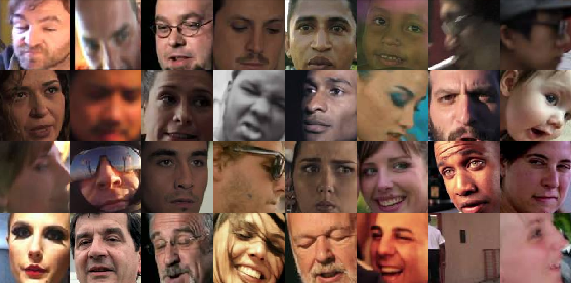
\includegraphics[width=0.98\linewidth]{img/random_sample_faces.png}
    \caption{A random selection of faces extracted from the dataset. In the bottom right corner we can see a false positive from extraction.}
    \label{fig:random_selection_faces}
\end{figure}

\section{Face similarity based on the deep features}

First of all, we were interested if the features from pretrained network contain interesting information, that could help in the search for a specific face. We used ... \todo[inline]{Add dlib more information}. This network produces a feature vector of length 128 as face representation. The authors' state, that the recommended threshold for euclidean distance for two feature vectors to be accepted as one is 0.6.

We investigated the results based on the euclidean distance and we show a result for a given face to find the closest (i.e., most similar) faces in the dataset. The sample can be seen in the figure \ref{fig:closest_faces}.


\begin{figure}
    \centering
    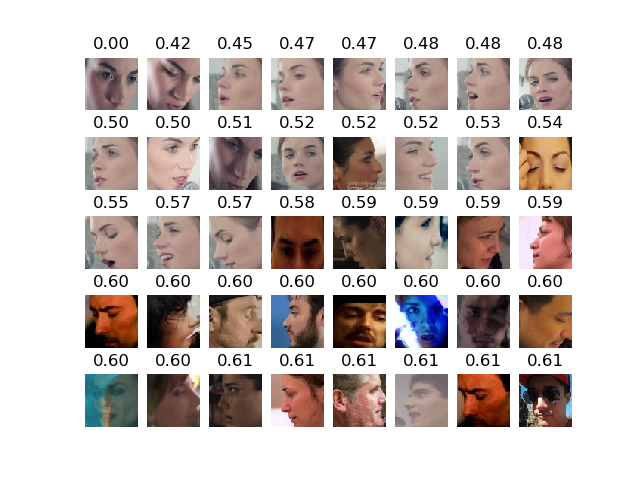
\includegraphics[width=\linewidth]{img/closest_faces_to_woman.png}
    \caption{Examples of the retrieved closest faces to the query face (top left) based on euclidean distance. Above images is the distance from the query.}
    \label{fig:closest_faces}
\end{figure}

\section{Case study}

The feature space we obtained in the previous steps was trained to identification task. Therefore, we wanted to find out, if the space over the face features contains also information about the similarity between the faces other than identification of the images of the same person.

We conducted a study with 25 participants. We presented them a grid $10\times10$ of randomly selected faces from the dataset. We then asked them, to select exactly three faces, which are the most similar to the provided target face. Our test contained 10 randomly pre-selected faces as the target. Two of the target faces were presented in the grid. This helped us to check, how likely is the user to see a face in a display with 100 faces.

Twenty-four out of 25 users selected the face corresponding to the same target person in the first case. In the second case, two face views of the target person were available in the grid. 9 respondents selected both correctly and 11 respondents selected only one of them. We conclude, that only in 70.7\% of the cases users noticed and correctly selected the target person in the grid.




\section{Building a search structure}

After examinating the features and their potential we created a hierarchical structure to give a possibility to examine more faces than the user can see at screen at once.


Our solution consists of the following steps, which are further described.
\begin{itemize}
    \item Find faces
    \item Compute face encoding
    \item Train self-organizing map (SOM) from the features
    \item Build layered structure over the SOM
\end{itemize}

\subsubsection*{Find Faces}
We use pretrained CNN face detector, which is available in Dlib from custom pretrained modell….


\subsubsection*{Compute face encodings}


\subsubsection*{Train self-organizing map from the features}
Train self-organizing map from the features
// popisat preco a co su self organizing maps



\subsubsection*{Build layered structure over the SOM}

In order to project the dataset to user we need add a new layer of options - nabigation. We have seen ... success with SOM 

By creating self-organizing map we layed down a grid lattice to include all available faces. This means that the size of the map corresponds to the size of the dataset. In our case, when we work with more than TODO faces, it is unbereable to present the user with all the faces at once.

We implement tree structure sampling. Each layer contains only a subset of faces available in the next layer. This representants are chosen as every k-th image from the next layer. In other words, our final model consists of n grid lattices. Ln-1 is the bottom layer containing the full SOM. Li for i e {0,...n-2} holds: Lixy = Li+1, x*k, y*k.
